\documentclass[12pt]{article}

\usepackage[sectionbib,authoryear,round]{natbib}
\usepackage{array,epsfig,fancyhdr,rotating}
\usepackage{amsmath,amssymb,amsfonts,amsthm,graphicx,booktabs,multirow,placeins}
\allowdisplaybreaks[1]
\usepackage{sectsty,secdot}
\usepackage{xr-hyper}
\usepackage[hidelinks]{hyperref}
\renewcommand{\bibsection}{\section*{References}}
\usepackage{etoolbox}
\AtBeginDocument{\apptocmd{\thebibliography}{\interlinepenalty=10000\clubpenalty=10000\widowpenalty=10000}{}{}}
\sectionfont{\fontsize{12}{14pt plus.8pt minus .6pt}\selectfont}
\subsectionfont{\fontsize{12}{14pt plus.8pt minus .6pt}\selectfont}
\textwidth=31.9pc
\textheight=46.5pc
\oddsidemargin=1pc
\evensidemargin=1pc
\headsep=15pt
\topmargin=.6cm
\parindent=1.7pc
\parskip=0pt
\emergencystretch=1em
\clubpenalty=10000
\widowpenalty=10000
\brokenpenalty=10000
\setcounter{page}{1}
\pagestyle{fancy}
\renewcommand{\sectionmark}[1]{}
\renewcommand{\subsectionmark}[1]{}
\lhead[\footnotesize\thepage\fancyplain{}\leftmark]{}
\chead[]{}
\rhead[]{\fancyplain{}\rightmark\footnotesize\thepage}
\cfoot{}
\fancypagestyle{firstpage}{\fancyhf{}\fancyhead[L]{\footnotesize\rm Statistica Sinica}\fancyhead[R]{\footnotesize\thepage}}
\newtheorem{theorem}{Theorem}
\newtheorem{lemma}{Lemma}
\newtheorem{corollary}{Corollary}
\newtheorem{proposition}{Proposition}
\newtheorem{assumption}{Assumption}
\newtheorem{step}{Step}
\newtheorem{setting}{Setting}
\newtheorem{definition}{Definition}
\newtheorem{example}{Example}
\newtheorem{remark}{Remark}

\newcommand{\ba}{{\mathbf a}}
\newcommand{\bb}{{\mathbf b}}
\newcommand{\be}{{\mathbf e}}
\newcommand{\bh}{{\mathbf h}}
\newcommand{\br}{{\mathbf r}}
\newcommand{\bu}{{\mathbf u}}
\newcommand{\bv}{{\mathbf v}}
\newcommand{\bx}{{\mathbf x}}
\newcommand{\bA}{{\mathbf A}}
\newcommand{\bB}{{\mathbf B}}
\newcommand{\bC}{{\mathbf C}}
\newcommand{\bD}{{\mathbf D}}
\newcommand{\bE}{{\mathbf E}}
\newcommand{\bG}{{\mathbf G}}
\newcommand{\bH}{{\mathbf h}}
\newcommand{\bI}{{\mathbf I}}
\newcommand{\bK}{{\mathbf K}}
\newcommand{\bL}{{\mathbf L}}
\newcommand{\bM}{{\mathbf M}}
\newcommand{\bQ}{{\mathbf Q}}
\newcommand{\bR}{{\mathbf R}}
\newcommand{\bS}{{\mathbf S}}
\newcommand{\bT}{{\mathbf T}}
\newcommand{\bU}{{\mathbf U}}
\newcommand{\bV}{{\mathbf V}}
\newcommand{\bW}{{\mathbf W}}
\newcommand{\bX}{{\mathbf X}}
\newcommand{\bY}{{\mathbf Y}}
\newcommand{\bZ}{{\mathbf Z}}
\newcommand{\bbeta}  {\boldsymbol{\beta}}
\newcommand{\btheta}  {\boldsymbol{\theta}}
\newcommand{\bmu} {\boldsymbol{{\mathbf \mu}}}
\newcommand{\bpsi} {\boldsymbol{{\mathbf \psi}}}
\newcommand{\bxi} {\boldsymbol{{\mathbf \xi}}}
\newcommand{\bGamma} {\boldsymbol{\Gamma}}
\newcommand{\bSigma} {\boldsymbol{\Sigma}}
\newcommand{\bPsi} {\boldsymbol{\Psi}}
\newcommand{\bPhi} {\boldsymbol{\Phi}}
\newcommand{\bXi} {\boldsymbol{\Xi}}
\newcommand{\bOmega} {\boldsymbol{\Omega}}
\newcommand{\bDelta} {\boldsymbol{\Delta}}
\newcommand{\real}{\mathbb{R}}
\newcommand{\expect}{\mathbb{E}}
\newcommand{\prob}{\mathbb{P}}
\newcommand{\Var}{\textrm{Var}}
\newcommand{\Cov}{\textrm{Cov}}
\newcommand{\diag}{\textrm{diag}}

\newcommand{\trans}{{\scriptscriptstyle\mathsf{T}}}
\newcommand{\wh}{\widehat}
\newcommand{\wt}{\widetilde}
\newcommand{\bone}{{\mathbf 1}}
\newcommand{\supp}{{\mathrm supp}}



\numberwithin{equation}{section}
\newcommand{\bodyfont}{\fontsize{12}{14pt plus.8pt minus .6pt}\selectfont}
\newcommand{\referencefont}{\bibhang=1.7pc\bibsep=2pt\fontsize{9}{14pt plus.8pt minus .6pt}\selectfont}
\externaldocument[][nocite]{fscb-supplement}

\begin{document}
\renewcommand{\baselinestretch}{2}
\bodyfont
\markboth{\hfill{\footnotesize\rm HAOZHEN SHU, ZHENHUA LIN AND YINAN LIN}\hfill}
{\hfill{\footnotesize\rm BANDS FOR FUNCTIONAL REGRESSION}\hfill}
\thispagestyle{firstpage}
$\ $\par\vspace{0.8pc}
\centerline{\large\bf SIMULTANEOUS CONFIDENCE BANDS FOR}
\vspace{2pt}
\centerline{\large\bf FUNCTIONAL VARYING-COEFFICIENT MODELS}
\vspace{.4cm}
\centerline{Haozhen Shu$^1$, Zhenhua Lin$^2$ and Yinan Lin$^3$}
\vspace{.4cm}
\centerline{\it $^1$National Institute of Education,}
\centerline{\it Nanyang Technological University,}
\centerline{\it $^2$National University of Singapore and}
\centerline{\it $^3$Chongqing Normal University}
\vspace{.55cm}

\fontsize{9}{11.5pt plus.8pt minus.6pt}\selectfont
\begin{quotation}
\noindent {\it Abstract:} We develop quantitative simultaneous inference for functional varying-coefficient models under sparse and dense sampling. A subject-level linear representation connects local polynomial estimation to high-dimensional Gaussian approximation without reconstructing individual trajectories. Explicit error bounds account for dimension, sampling frequency, smoothing bias, estimated designs, and fitted residuals. A Gaussian multiplier bootstrap calibrates joint confidence bands over time and coefficients. The theory allows growing regression dimension and yields joint bands for high-dimensional mean functions under polynomial moment conditions. Simulations and a liver-disease biomarker analysis illustrate the procedure.
\par
\vspace{9pt}
\noindent {\it Key words and phrases:} Functional data, Gaussian approximation, multiplier bootstrap, simultaneous inference, varying-coefficient model.
\end{quotation}
\bodyfont
\section{Introduction}\label{sec:intro}

Simultaneous inference for functional data requires uncertainty to be controlled over an entire time interval and, for multivariate targets, across several functions at once. This problem is particularly challenging under sparse and irregular sampling, when individual trajectories cannot be accurately reconstructed from their own measurements. Varying-coefficient models (VCMs) provide an important setting: they describe associations that evolve over time through a vector of coefficient functions \citep{hastie_tibshirani_1993,gu_et_al_2014,cao_simultaneous_2018}. Joint confidence bands must account for dependence within subjects and across coefficient estimates, while remaining valid as the number of observations per subject increases. We study this problem through quantitative Gaussian and bootstrap approximation, with explicit control of the errors that determine simultaneous coverage.

The sampling design has long been central to functional data analysis; see \citet{wang_functional_2016}. Dense-data inference can exploit accurate trajectory reconstruction \citep{zhang_chen_2007}, whereas sparse-data methods pool information across subjects \citep{yao_functional_2005}. Uniform estimation theory and optimal mean-estimation rates clarify the transition between these settings \citep{li_hsing_2010,cai_optimal_2011}. \citet{zhang_wang_2016} also distinguish equal-subject and equal-observation weighting when counts differ. These choices change how sampling frequency enters the variance and cannot be interchanged without checking the resulting theory.

Simultaneous inference is available in both classical regimes. For mean curves, dense-data bands include \citet{degras_2011,cao_yang_todem_2012}, and sparse-data bands include \citet{ma_yang_carroll_2012,zheng_smooth_2014}. For regression, local polynomial and spline methods provide established estimation and inference tools \citep{wu_chiang_2000,huang_wu_zhou_2004,fan_simultaneous_2000}. \citet{gu_et_al_2014} develop sparse-data coefficient bands with time-independent covariates, while \citet{cao_simultaneous_2018} allow time-varying covariates under sparse irregular sampling. Dense functional-response regression is studied by \citet{zhu_li_kong_2012,chang_lin_ogden_2017}. \citet{zhou_el_2024} develop empirical-likelihood M-estimation and simultaneous regions for functional responses with subject-level covariates observed on a common grid. More recently, \citet{chang_mckeague_2024} construct empirical-likelihood bands for concurrent regression on a dense fixed grid, allowing nonsmooth functional features. These dense-grid results and sparse random-design results address different observation schemes.

Several inferential methods accommodate a range of observation frequencies. \citet{kim_zhao_2013} study longitudinal mean inference, \citet{chen_yao_2017} develop self-normalized pointwise inference for varying coefficients, and \citet{wang_et_al_2018} provide empirical-likelihood pointwise regions and global tests for concurrent functional regression. These pointwise and global procedures address different inferential targets from bands calibrated jointly over time and coefficient functions.

For scalar mean functions, \citet{cai_hu_2025} and \citet{LouWu2026} develop unified simultaneous inference using B-spline and local linear estimators, respectively. Their Gaussian approximations yield asymptotically valid bands and characterize covariance transitions across sampling frequencies. Our focus is quantitative simultaneous inference for vector-valued functional parameters throughout this transition.

We take a nonasymptotic approach based on high-dimensional Gaussian approximation and comparison theory \citep{chernozhukov_central_2017,chernozhukov_et_al_2022}. Representing the estimation error through independent subject contributions allows us to analyze sparse observations without reconstructing individual trajectories. We derive explicit bounds for Gaussian approximation, conditional bootstrap approximation, and joint coverage error. These bounds quantify how sample size, dimension, observation frequency, and bandwidth determine inferential accuracy, providing a quantitative explanation of the sparse-to-dense phase transition and distinguishing its consequences for approximation error and band width.

A Gaussian multiplier bootstrap calibrates the joint maximum directly from fitted subject contributions, avoiding separate estimation of the functional-error covariance surface or selection of a sampling regime. We establish its validity while accounting for fitted residuals, estimated design matrices, and studentization. The framework accommodates local polynomial estimators of any fixed degree and yields joint bands for VCMs with random time-varying predictors and growing dimension. An intercept-only specialization yields joint bands over time and a growing collection of mean functions with coordinate-specific errors. Its rates depend on dimension through logarithmic factors and a maximum-coordinate tail envelope.

Section~\ref{sec:method} introduces the model, estimator, and regularity conditions. Section~\ref{sec:theory} develops the linear representation, Gaussian and bootstrap approximation, simultaneous bands, and a high-dimensional mean corollary. Section~\ref{sec:numerical-study} reports simulations and an exploratory Mayo PBC analysis. The Supplementary Material provides proofs, additional sampling-frequency and mean results, and bandwidth and implementation details.

\section{Model and regularity conditions}\label{sec:method}

\subsection{Model and estimation}\label{sec:model}\label{sec:estimation}

Let $Y_i(t)$ be a scalar response and
$\bX_i(t)=\{X_{i1}(t),\ldots,X_{ip}(t)\}^\trans$ a vector of predictors
for subject $i$ at time $t\in\mathcal T=[0,1]$.
We consider the functional varying-coefficient model
\begin{equation}
Y_i(t)=\bX_i(t)^\trans\bbeta(t)+\varepsilon_i(t),
\qquad i=1,\ldots,n,
\label{eq:model-VCM-pop}
\end{equation}
where $\bbeta(t)=\{\beta_1(t),\ldots,\beta_p(t)\}^\trans$ is a vector of
unknown coefficient functions and $\varepsilon_i(t)$ is a functional
error process. The coefficient $\beta_k(t)$ describes the linear
association between the response and the $k$th predictor at time $t$,
with the other predictors included in the model. A constant coordinate
$X_{i1}(t)\equiv1$ supplies an intercept; time-independent covariates can
likewise be included as constant coordinate processes. Both the predictors
and their associations with the response may vary over time, and the
dimension $p=p_n$ may increase with $n$.

The subject processes are independent across $i$, while dependence within
a subject is retained. We impose the pointwise orthogonality condition
$\expect\{\bX_i(t)\varepsilon_i(t)\}=\mathbf0$.
Writing $\bOmega(t)=\expect\{\bX_i(t)\bX_i(t)^\trans\}$, this condition
identifies the population linear regression coefficient as
$\bbeta(t)=\bOmega(t)^{-1}\expect\{\bX_i(t)Y_i(t)\}$
whenever $\bOmega(t)$ is nonsingular. In particular, this formulation
does not require the predictor and error processes to be independent.

The trajectories are observed at subject-specific times. Subject $i$
supplies $(T_{ij},\bX_{ij},Y_{ij})$, $j=1,\ldots,m_i$, where
$\bX_{ij}=\bX_i(T_{ij})$, $Y_{ij}=Y_i(T_{ij})$, and
$\varepsilon_{ij}=\varepsilon_i(T_{ij})$.
The observation times have a common density $f$ and are independent of
the subject processes. The counts $m_i$ may differ across subjects and
may remain bounded or increase with $n$. We pool observations across
subjects for estimation and simultaneous inference over all
$t\in\mathcal T$ and all $p$ coefficient functions, without first
reconstructing individual trajectories.

To construct a local polynomial estimator, fix a degree $r\ge0$ and a
bandwidth $h>0$. At every target time $t\in\mathcal T$, approximate each
coefficient function by its Taylor polynomial in
a neighborhood of $t$. Under the smoothness condition in
Assumption~\ref{ass:design},
\[
\beta_k(v)=\sum_{a=0}^r\frac{h^a\beta_k^{(a)}(t)}{a!}
\left(\frac{v-t}{h}\right)^a+O(|v-t|^{r+1}),
\qquad |v-t|\le h,
\]
where $v\in\mathcal T$, $\beta_k^{(0)}=\beta_k$, and the remainder
bound is uniform in $k$ and $t$.
Thus the coefficient of the normalized power $\{(v-t)/h\}^a$
approximates $h^a\bbeta^{(a)}(t)/a!$.
The polynomial approximation concerns the coefficient functions; the
predictors enter through their observed values $\bX_{ij}$.

Let $K$ be a nonnegative kernel supported on $[-1,1]$ and put
$K_h(u)=K(u/h)/h$. Define
\[
\btheta_r(u)=(1,u,\ldots,u^r)^\trans,\qquad
\bpsi_{ij}(t)=\btheta_r\{(T_{ij}-t)/h\}\otimes\bX_{ij},
\]
where $\otimes$ denotes the Kronecker product.
Write the local polynomial coefficients as a block vector
$\bb=(\bb_0^\trans,\ldots,\bb_r^\trans)^\trans\in\real^{(r+1)p}$.
The corresponding local predictor is
\[
\bpsi_{ij}(t)^\trans\bb
=\sum_{a=0}^r\bX_{ij}^\trans\bb_a
\left(\frac{T_{ij}-t}{h}\right)^a.
\]
We estimate the blocks by equal-subject weighted least squares:
\begin{equation}
\wh\bb(t)=\arg\min_{\bb\in\real^{(r+1)p}}
\frac1n\sum_{i=1}^n\frac1{m_i}\sum_{j=1}^{m_i}
K_h(T_{ij}-t)\{Y_{ij}-\bpsi_{ij}(t)^\trans\bb\}^2.
\label{eq:local-polynomial-fit}
\end{equation}
The kernel localizes the fit to observations within distance $h$ of $t$.
The factor $1/m_i$ first averages the losses within each subject, so that
every subject receives the same total weight before localization. This
weighting keeps subjects with more observations from receiving greater
total weight solely because of their observation counts.

For computation, define the empirical design matrix
\[
\wh{\bD}_h(t)=n^{-1}\sum_i m_i^{-1}\sum_j
K_h(T_{ij}-t)\bpsi_{ij}(t)\bpsi_{ij}(t)^\trans
\]
and its population counterpart $\bD_h(t)=\expect\{\wh{\bD}_h(t)\}$.
When $\wh{\bD}_h(t)$ is invertible, the normal equations for
\eqref{eq:local-polynomial-fit} give
\[
\wh\bb(t)=\wh{\bD}_h(t)^{-1}
\frac1n\sum_{i=1}^n\frac1{m_i}\sum_{j=1}^{m_i}
K_h(T_{ij}-t)\bpsi_{ij}(t)Y_{ij}.
\]
Partition $\wh\bb(t)$ into its $p$-dimensional blocks
$\wh\bb_0(t),\ldots,\wh\bb_r(t)$. Evaluating the fitted polynomial at
its center gives $\wh\bbeta(t)=\wh\bb_0(t)=\bL\wh\bb(t)$, where
$\bL=[\bI_p\ \mathbf0\ \cdots\ \mathbf0]$.

The same fit also supplies derivative estimators. Differentiating the
fitted polynomial with respect to its time argument and evaluating at
$t$ yields
\begin{equation}
\wh\bbeta^{(a)}(t)=\frac{a!}{h^a}\wh\bb_a(t),
\qquad a=0,\ldots,r,
\label{eq:local-polynomial-derivatives}
\end{equation}
with $\wh\bbeta^{(0)}=\wh\bbeta$.
For local linear fitting ($r=1$), the first two blocks estimate
$\bbeta(t)$ and $h\bbeta'(t)$, respectively, so that
$\wh\bbeta'(t)=\wh\bb_1(t)/h$. For $r\ge2$, the second derivative is
estimated by $2\wh\bb_2(t)/h^2$. The notation in
\eqref{eq:local-polynomial-derivatives} refers to derivatives of the
local fitted polynomial at its center; these estimators need not equal
derivatives of the curve obtained by moving the fitting center $t$.
The simultaneous bands developed below concern the coefficient functions
corresponding to $a=0$.

\subsection{Regularity conditions}\label{sec:conditions}

We first collect the notation used in the assumptions and results.
For a vector $x$, $\|x\|_2$ is its Euclidean norm and
$\|x\|_\infty$ is its largest absolute coordinate. For a vector-valued
function $g$ and a time set $I\subseteq\mathcal T$, write
$\|g\|_{a,I}=\sup_{t\in I}\|g(t)\|_a$, $a\in\{2,\infty\}$.
The first subscript specifies the pointwise vector norm; the second
specifies the time set over which the supremum is taken. Thus $\|\wh\bbeta-\bbeta\|_{\infty,\mathcal T}$ measures the largest
absolute estimation error over all coefficients and times, whereas
$\|\wh\bbeta-\bbeta\|_{2,\mathcal T}$ measures the largest Euclidean
error over time.

For a matrix-valued function $A$, $\|A\|_{\infty,I}$ denotes the largest
absolute entry maximized over $I$; the same convention applies to
functions of two time arguments on $I^2$. We use
$\|\cdot\|_{\mathrm{op}}$ for the spectral norm and $\preceq$ for the
positive-semidefinite order. For a scalar random variable $Z$,
$\|Z\|_{L^q}=\{\expect(|Z|^q)\}^{1/q}$ denotes its moment norm.
We write $\mathcal F_n$ for the sigma-field generated by all
observations and state conditional probabilities and expectations
explicitly given $\mathcal F_n$.

The dimension $p=p_n$ may grow, while the polynomial degree $r$ and
moment order $q\ge4$ are fixed. Constants in the assumptions and in
the $\lesssim$ and $O_P$ bounds are independent of $n,p,h$ and the
observation counts.
All processes are assumed jointly measurable and separable, and all
suprema below are measurable. All time-indexed conditions hold uniformly
over $\mathcal T=[0,1]$.

\begin{assumption}[Sampling]\label{ass:core}
For each $n$, the pairs $(\bX_i,\varepsilon_i)$ are independent and
identically distributed across subjects, and the counts $m_i\ge1$
are deterministic. Their common process law may depend on $n$.
The times $T_{ij}$ are mutually independent with common density $f$,
and independent of the subject processes. The model
\eqref{eq:model-VCM-pop} satisfies
$\expect\{\bX(t)\varepsilon(t)\}=\mathbf0$ for all $t$.
\end{assumption}

\begin{assumption}[Smoothness and identification]\label{ass:design}
The coordinates of $\bbeta$ belong to a common bounded
$C^{r,1}(\mathcal T)$ class: they have $r$ continuous derivatives,
and their $r$th derivatives are Lipschitz; for $r=0$, the functions
themselves are Lipschitz. The density $f$ is Lipschitz and
$0<c_f\le f\le C_f$. With
$\bOmega(t)=\expect\{\bX(t)\bX(t)^\trans\}$,
\[
c_\Omega\bI_p\preceq\bOmega(t)\preceq C_\Omega\bI_p,
\qquad
\|\bOmega(t)-\bOmega(u)\|_{\mathrm{op}}\le C|t-u|.
\]
\end{assumption}

\begin{assumption}[Kernel and bandwidth]\label{ass:kernel}
The kernel $K$ is nonnegative, symmetric, Lipschitz on $\mathbb R$,
supported on $[-1,1]$, and has integral one. The bandwidth is
deterministic, $0<h\le1/2$, and $h\to0$.
\end{assumption}

\begin{assumption}[Coordinate moments]\label{ass:moments}
For a fixed $q\ge4$,
\[
\max_{k\le p}\expect\{\sup_t|X_k(t)|^{2q}\}
+\max_{k\le p}\expect\{\sup_t|X_k(t)\varepsilon(t)|^q\}\le C.
\]
Write $F_i=\sup_t\|\bX_i(t)\|_\infty^2+
\sup_t\|\bX_i(t)\varepsilon_i(t)\|_\infty$ and assume
$\|F_i\|_{L^q}\le K_n$.
The coordinate moment bounds yield the worst-case upper bound
$\|F_i\|_{L^q}\le Cp^{1/q}$, and we can take $1\le K_n\le Cp^{1/q}$. Stronger assumptions that yield smaller
$K_n$ lead to sharper rates.
\end{assumption}

\begin{assumption}[Score covariance]\label{ass:covariance}
The score covariance kernel
$\bC(u,v)=\expect\{\bX(u)\varepsilon(u)\varepsilon(v)\bX(v)^\trans\}$
satisfies $\sup_{u,v}\|\bC(u,v)\|_{\mathrm{op}}\le C$ and
\[
\|\bC(u,v)-\bC(u',v')\|_{\mathrm{op}}
\le C(|u-u'|+|v-v'|).
\]
For $\bV_F(t)=\bOmega(t)^{-1}\bC(t,t)\bOmega(t)^{-1}$,
$\inf_{t\in\mathcal T}\min_{k\le p}[\bV_F(t)]_{kk}\ge c_F>0$.
\end{assumption}

Assumptions~\ref{ass:core}--\ref{ass:kernel} describe independently
sampled subjects with noninformative random observation times, smooth
coefficients, and a uniformly well-conditioned design, while retaining
within-subject dependence. Examples include well-conditioned banded
second-moment matrices with uniformly Lipschitz entries and a fixed
number of nonzero diagonals, and the Epanechnikov kernel used in our
numerical studies.

Assumptions~\ref{ass:moments}--\ref{ass:covariance} accommodate growing
dimension, polynomial tails of sufficiently high order, and dependence
across times and coordinates, with $K_n$ recording the size of the
largest-coordinate envelope. The coordinate variance condition holds,
for example, for mean-zero functional errors independent of the
predictors with uniformly positive variances. The general condition
also allows singular score covariance matrices.

\section{Simultaneous inference}\label{sec:theory}

Simultaneous coverage requires control of the maximum absolute standardized
estimation error over time and coefficient functions. Establishing the
validity of the bands therefore requires both an approximation to the
distribution of this maximum and a way to estimate its critical value
from the observed data. We proceed in three steps. First, we derive a
uniform linear representation that expresses the estimation error as a
sum of independent subject contributions plus a controlled remainder.
This representation retains within-subject dependence and separates the
leading stochastic variation from smoothing bias and error in the
estimated local design. Second, we approximate the joint maximum by its
Gaussian counterpart and examine how sampling frequency affects the
approximation error across sparse and dense designs. Third, we show
that a feasible subject multiplier bootstrap reproduces this reference
distribution, accounting for fitted residuals and estimated standard
errors, and use its conditional quantile to calibrate the joint bands.
The resulting coverage and band-width bounds clarify how repeated
measurements affect simultaneous inference. We then specialize the
construction to multiple mean functions with coordinate-specific errors.

\subsection{Linear representation}\label{sec:theory-linear}

Define the subject score and its population-weighted contribution by
\begin{equation*}
\bu_i(t)=\frac1{m_i}\sum_{j=1}^{m_i}
K_h(T_{ij}-t)\bpsi_{ij}(t)\varepsilon_{ij},
\qquad \bPsi_i(t)=\bL\bD_h(t)^{-1}\bu_i(t).
\end{equation*}
The $\bPsi_i$ are independent and centered. Put $s=r+1$ and
\begin{gather}
\kappa_{a,n}=\frac1n\sum_{i=1}^n m_i^{-a}\quad(a=1,3),\qquad
v_n^2=1+\frac{\kappa_{1,n}}h,\qquad L_n=\log(np/h),\notag\\
\delta_n=v_n\sqrt{\frac{L_n}{n}}+
\frac{K_n L_n}{n^{1-1/q}h},\notag\\
\rho_n=p^{q/(2q-2)}v_n\sqrt{\frac{L_n}{n}}
+\frac{pL_n}{n^{1-1/q}h}.
\label{eq:basic-rates}
\end{gather}
Here $K_n\ge1$ bounds the $L^q$ norm of the largest coordinate design and
score envelope, defined in Assumption~\ref{ass:moments}.
The scale $v_n^2$ is the order of the average coordinate variance of the
subject contributions. The rate $\delta_n$ controls score coordinates,
whereas $\rho_n$ controls the empirical design in spectral norm.
Direct matrix moment bounds give $\rho_n\lesssim p\delta_n$.
The matrix envelope has $L^q$ norm of order at most $p$, directly
from the coordinate moments.

\begin{theorem}[Uniform linear representation]\label{thm:linear}
Under Assumptions~\ref{ass:core}--\ref{ass:moments}, if $\rho_n\to0$,
the empirical design is uniformly invertible on $\mathcal T$ with
probability tending to one, and
\begin{equation*}
\wh\bbeta(t)-\bbeta(t)=\frac1n\sum_{i=1}^n\bPsi_i(t)+\bR_n(t),
\qquad t\in\mathcal T,
\end{equation*}
where
\begin{align*}
\|\wh\bbeta-\bbeta\|_{2,\mathcal T}
&=O_P\{\sqrt p(\delta_n+h^s)\},\\
\|\bR_n\|_{\infty,\mathcal T}
&=O_P\{\sqrt p(\rho_n\delta_n+h^s)\}.
\end{align*}
\end{theorem}

The remainder accounts for estimation of the local design and smoothing
bias. When the variance terms dominate in $\rho_n$ and $\delta_n$,
its stochastic component is
$O_P\{p^{1+1/(2q-2)}v_n^2L_n/n\}$.
The factor $\sqrt p$ in the bias bound reflects coordinatewise
smoothness of the $p$ coefficient functions. The bounds hold over the
full fitting interval, so they also control the coefficient estimates
used to form residuals at the observed times.

The explicit powers of $p$ arise from worst-case bounds under the stated
moment and smoothness assumptions. In particular, the inverse local
design can combine errors from many coordinates, and the analysis
controls this effect without imposing sparsity or a block structure.
Stronger structural assumptions on the predictors or the local design
may yield smaller dimension factors. For example, well-conditioned
block-diagonal designs with uniformly bounded block sizes limit the
number of coordinates combined by the inverse design and may permit
sharper rates through a refined analysis. The displayed dependence on
$p$ therefore gives sufficient bounds for the general model.

For simultaneous inference, the key consequence of
Theorem~\ref{thm:linear} is the reduction of the estimation error to a
sum of independent, centered subject processes with a quantified
remainder. This form allows Gaussian approximation to be applied at
the subject level while retaining dependence within each subject. The
uniform remainder bound then quantifies the error in transferring that
approximation to the maximum of the standardized coefficient errors
over time. The next subsection carries out this comparison, with design
estimation and smoothing bias entering explicitly into the Gaussian
approximation bound.

\subsection{Gaussian approximation}\label{sec:theory-gaussian}

Let $\tau_k^2(t)=n^{-1}\sum_i\expect\{\Psi_{ik}^2(t)\}$ and let $G_n$ be a
centered continuous Gaussian process with
\begin{equation*}
\expect\{G_{n,k}(u)G_{n,l}(t)\}=
\frac{\sum_{i=1}^n\expect\{\Psi_{ik}(u)\Psi_{il}(t)\}}
{n\tau_k(u)\tau_l(t)}.
\end{equation*}
Under Assumption~\ref{ass:covariance}, $\tau_k(t)\asymp v_n$ uniformly;
the covariance calculation is in Section~\ref{app:covariance-proof}.
For comparison with $S_{G,n}=\|G_n\|_{\infty,\mathcal T}$, define
\[
T_n^\circ=\sup_{t\in\mathcal T}\max_{k\le p}
\frac{\sqrt n\,|\wh\beta_k(t)-\beta_k(t)|}{\tau_k(t)}.
\]
Set $T_n^\circ=0$ on the exceptional design event.
Define the moment scales and the Gaussian approximation error by
\begin{align}
\Lambda_n&=\frac{1+\kappa_{3,n}/h^3}{v_n^4},\qquad
B_n=\max\left\{\frac{\sqrt p\,K_n}{hv_n},p\sqrt{\Lambda_n}\right\},\notag\\
\gamma_n&=\left(\frac{B_n^2L_n^5}{n}\right)^{1/4}
+\frac{B_nL_n^{3/2-1/q}}{n^{1/2-1/q}}\notag\\*
&\quad+\left(\frac{\sqrt{npL_n}\,\rho_n\delta_n}{v_n}\right)^{1/2}
+\frac{\sqrt{npL_n}\,h^s}{v_n}.
\label{eq:gaussian-rate}
\end{align}

\begin{theorem}[Gaussian approximation]\label{thm:gaussian}
Under Assumptions~\ref{ass:core}--\ref{ass:covariance}, if
$\rho_n\to0$, then, for all sufficiently large $n$,
\begin{equation*}
\sup_z\left|\prob(T_n^\circ\le z)-\prob(S_{G,n}\le z)\right|
\le C\gamma_n.
\end{equation*}
\end{theorem}

The first two terms of $\gamma_n$ control Gaussian approximation of
the subject scores; the remaining terms account for design estimation
and smoothing bias. Smaller discretization and exceptional-event terms
are absorbed into this bound, as shown in the proof.

\noindent\textbf{Phase transition for the CLT.}
Theorem~\ref{thm:gaussian} gives a quantitative central limit theorem
(CLT) for the joint maximum. To examine how its approximation error
changes with sampling frequency, consider fixed $p$ and balanced
observation counts $m_i=m$. Then $K_n=O(1)$ and the coordinate standard
errors have order $\{n^{-1}+(nmh)^{-1}\}^{1/2}$. The following
corollary makes this dependence explicit.

\begin{corollary}[Gaussian approximation across sampling frequencies]
\label{cor:fixedp-phase}
Under Assumptions~\ref{ass:core}--\ref{ass:covariance}, take fixed $p$,
$m_i=m$, and $q>4$. Suppose $h\ge n^{-C}$ for some fixed $C>0$, and
\begin{equation}
\begin{aligned}
n\wedge(nmh)&\gtrsim n^{4/q}(\log n)^{3-4/q},\\
\{n\wedge(nmh)\}^{3/4}h^s&\lesssim(\log n)^{5/4}.
\end{aligned}
\label{eq:fixedp-phase-conditions}
\end{equation}
Then, for all sufficiently large $n$,
\begin{equation}
\begin{aligned}
&\sup_z\left|\prob(T_n^\circ\le z)-\prob(S_{G,n}\le z)\right|\\
&\quad\le C\left\{\frac{\log^7 n}{n\wedge(nmh)}\right\}^{1/4}.
\end{aligned}
\label{eq:fixedp-phase-clt}
\end{equation}
\end{corollary}

The first balance in \eqref{eq:fixedp-phase-conditions} makes the
finite-moment term no larger than the Gaussian approximation term;
the second places smoothing bias below the same bound. These are
sufficient simplifications of the general rates. They hold, for
example, for $q=8$, $r\ge1$, and $h=n^{-2/5}$ for every $m\ge1$.
Section~\ref{app:refined-sampling-bounds} gives the derivation.

When $mh\le1$, the bound is
$\{\log^7 n/(nmh)\}^{1/4}$, whereas $mh\ge1$ gives
$(\log^7 n/n)^{1/4}$. Thus the effective sample size increases with
the number $nmh$ of observations in local windows and reaches the
order of the number $n$ of independent subjects at $mh\asymp1$.
The reference Gaussian law retains the corresponding covariance
throughout this transition. The implications for band width are
considered in Section~\ref{sec:SCB}, after the bands are constructed.

\subsection{Bootstrap approximation}\label{sec:theory-bootstrap}

We now return to the general setting in which $p$ may grow with $n$.
Theorem~\ref{thm:gaussian} provides a reference distribution for the
maximum standardized estimation error across sampling frequencies.
Using this reference law for calibration
requires estimating the unknown covariance of the subject contributions
and the normalizing variances $\tau_k^2(t)$. We address this through a
subject multiplier bootstrap based on fitted contributions.
Conditionally on the observations, the multiplier process is Gaussian,
with covariance determined by empirical products of these contributions.
It therefore provides a way to approximate the reference law from the
data while retaining dependence across time and coefficients, without
separately estimating the functional-error covariance surface. To
justify this step, we must control the effects of replacing population
designs and errors by estimated designs and fitted residuals, as well
as the effect of estimating the normalizing variances.

To construct the bootstrap, form $\wh\varepsilon_{ij}
=Y_{ij}-\bX_{ij}^\trans\wh\bbeta(T_{ij})$ and
\begin{equation*}
\begin{split}
\wh\bPsi_i(t)&=\bL\wh{\bD}_h(t)^{-1}\frac1{m_i}
\sum_{j=1}^{m_i}K_h(T_{ij}-t)\bpsi_{ij}(t)\wh\varepsilon_{ij},\\
\wh\sigma_k^2(t)&=\frac1n\sum_{i=1}^n\wh\Psi_{ik}^2(t).
\end{split}
\end{equation*}
Independently of the data, draw independent $\xi_i\sim N(0,1)$ and set
\begin{equation*}
G_{n,k}^*(t)=\frac1{\sqrt n}\sum_{i=1}^n
\xi_i\frac{\wh\Psi_{ik}(t)}{\wh\sigma_k(t)},\qquad
S_n^*=\|G_n^*\|_{\infty,\mathcal T}.
\end{equation*}
A single multiplier is shared by all observations and coordinates of a
subject. The statistic being calibrated is
\[
T_n=\sup_{t\in\mathcal T}\max_{k\le p}
\frac{\sqrt n\,|\wh\beta_k(t)-\beta_k(t)|}{\wh\sigma_k(t)}.
\]
Collect the covariance and fitted-score errors in
\begin{equation}
e_n=p\left\{\sqrt{\frac{\Lambda_nL_n}{n}}
+\frac{K_n^2L_n}{n^{1-2/q}h^2v_n^2}
+\sqrt p(\delta_n+h^s)\right\}.
\label{eq:bootstrap-covariance-scales}
\end{equation}
On samples with a singular local design or a nonpositive fitted variance,
set $T_n,S_n^*,G_n^*$ to zero and the bands to the empty set.
The oracle statistic $T_n^\circ$ keeps its earlier convention.
The proofs include the probability of these exceptional samples.
The first two terms in $e_n$ control empirical covariance fluctuations;
the last accounts for replacing the population-weighted subject scores
by contributions computed from estimated designs and fitted residuals.
The following theorem controls the resulting distributional errors when
the same observations are used for estimation and calibration.

\begin{theorem}[Bootstrap approximation]\label{thm:bootstrap}
Under Assumptions~\ref{ass:core}--\ref{ass:covariance}, if $e_n\to0$,
then
\begin{align*}
\sup_z\left|\prob(S_n^*\le z\mid\mathcal F_n)
-\prob(S_{G,n}\le z)\right|
&=O_P(\sqrt{e_n}\,L_n),
\\
\sup_z\left|\prob(T_n\le z)
-\prob(S_n^*\le z\mid\mathcal F_n)\right|
&=O_P(\gamma_n+\sqrt{e_n}\,L_n).
\end{align*}
\end{theorem}

The first bound shows that the conditional bootstrap distribution
approximates the Gaussian reference law from
Theorem~\ref{thm:gaussian}. The second connects this conditional law
to the sampling distribution of $T_n$, which uses estimated standard
errors. Together, the bounds account for both the Gaussian approximation
error $\gamma_n$ and the additional error from estimated subject
contributions and variance normalization. Both distributional errors
vanish in probability if $\gamma_n\to0$ and $e_nL_n^2\to0$.
These conditions specify how dimension, sampling frequency, and
bandwidth may vary jointly, allowing $p$ to increase with $n$.

The bootstrap distribution can therefore be used to estimate a common
critical value for the maximum error over all times and coefficients.
Passing from this distributional comparison to a coverage guarantee
also requires accounting for the randomness of the critical value,
which is computed from the same observations as the coefficient
estimates. The next subsection constructs the bands from a conditional
bootstrap quantile and uses a quantile bracket to obtain an explicit
bound on their joint coverage error.

\subsection{Simultaneous confidence bands}\label{sec:SCB}

For $v\in(0,1)$, define the conditional quantile
\begin{equation}
\wh q_v=\inf\{z:\prob(S_n^*\le z\mid\mathcal F_n)\ge v\}.
\label{eq:method-bootstrap-quantile}
\end{equation}
At confidence level $1-\alpha$, the bands are
\begin{equation*}
\mathcal C_{1-\alpha,k}(t)=
\left[\wh\beta_k(t)\ \pm\
\frac{\wh q_{1-\alpha}\wh\sigma_k(t)}{\sqrt n}\right],
\qquad t\in\mathcal T,\quad k=1,\ldots,p.
\end{equation*}
The common critical value calibrates coverage jointly over time and
coefficient functions.

\begin{theorem}[Simultaneous coverage]\label{thm:coverage}
Under Assumptions~\ref{ass:core}--\ref{ass:covariance}, suppose
$\gamma_n\to0$ and $e_nL_n^2\to0$. For every fixed $\alpha\in(0,1)$,
\begin{equation*}
\begin{split}
\Big|\prob\{\beta_k(t)\in\mathcal C_{1-\alpha,k}(t)
\text{ for all }t\in\mathcal T,\ k\le p\}-(1-\alpha)\Big|\\
\le C\{\gamma_n+(e_nL_n^2)^{1/3}\}.
\end{split}
\end{equation*}
\end{theorem}

The bands use the uncorrected local polynomial estimate, so the bandwidth
must make smoothing bias negligible for simultaneous inference. In
particular, $\gamma_n\to0$ includes the undersmoothing requirement
\begin{equation}
\frac{\sqrt{npL_n}\,h^{r+1}}{v_n}\to0.
\label{eq:vcm-undersmoothing}
\end{equation}
The uniform bias bound is $O(\sqrt p\,h^{r+1})$, and the coordinate
standard errors have order $v_n/\sqrt n$. The additional factor
$\sqrt{L_n}$ controls the effect of this bias on the distribution of the
joint maximum. The remaining terms of $\gamma_n$ and $e_n$ also restrict
how small $h$ may be. The multiplier bootstrap calibrates stochastic
fluctuations; the displayed bandwidth condition controls smoothing bias.

The coverage bound follows from a probability bound for covariance error
and a bracket for the random critical value. In practice, $\wh q_{1-\alpha}$
is approximated by the empirical quantile of independent multiplier draws.

\noindent\textbf{Phase transition for band width.}
With the bands defined, we return to the fixed-dimensional,
balanced-sampling setting of Corollary~\ref{cor:fixedp-phase}.
The following specialization establishes joint coverage in this setting
and describes how repeated measurements affect band width.

\begin{corollary}[Coverage and band width across sampling frequencies]
\label{cor:fixedp-width}
Under the conditions of Corollary~\ref{cor:fixedp-phase}, for every fixed
$\alpha\in(0,1)$, the bands have simultaneous coverage tending to
$1-\alpha$. Their half-widths
$w_{n,k}(t)=\wh q_{1-\alpha}\wh\sigma_k(t)/\sqrt n$ satisfy, with
probability tending to one, uniformly for $t\in\mathcal T$ and $k\le p$,
\begin{equation}
c\left\{\frac1{\sqrt n}+\sqrt{\frac{\log(1/h)}{nmh}}\right\}
\le w_{n,k}(t)\le
C\left\{\frac1{\sqrt n}+\sqrt{\frac{\log(1/h)}{nmh}}\right\}.
\label{eq:fixedp-phase-width}
\end{equation}
\end{corollary}

The proof of Corollaries~\ref{cor:fixedp-phase} and~\ref{cor:fixedp-width}
is given in Section~\ref{app:refined-sampling-bounds}.

Band width gives a complementary perspective on the transition. When
$mh\ll\log(1/h)$, the half-width has order
$\{\log(1/h)/(nmh)\}^{1/2}$; when $mh\gtrsim\log(1/h)$, it has
order $n^{-1/2}$. The additional logarithm is the cost of simultaneous
coverage over time. Consequently, the crossover for band width occurs
later than the crossover for coordinate variance.

Repeated measurements reduce the uncertainty from observing a
trajectory at finitely many times. They continue to share the same
subject-specific functional error, however, so increasing their number
cannot remove variation between subjects. Once the local sampling
contribution is small, further visits mainly resolve an already
observed trajectory and yield diminishing improvements in inference.
Increasing the number of independent subjects reduces the remaining
uncertainty and narrows the bands beyond this plateau.

\subsection{An extension to high-dimensional mean functions}
\label{sec:mean-model}

A natural corollary of the preceding VCM argument concerns simultaneous
inference for a growing collection of mean functions. Each mean is the
coefficient function in a VCM whose sole predictor is identically equal
to one. Applying this specialization coordinatewise gives
\[
Y_{ij,k}=\mu_k(T_{ij})+\varepsilon_{i,k}(T_{ij}),
\qquad j\le m_i,\quad k\le p.
\]
Retain the observation design, kernel, bandwidth, and measurability
conditions of Section~\ref{sec:conditions}. The mean-zero error processes
$(\varepsilon_{i,1},\ldots,\varepsilon_{i,p})^\trans$ are i.i.d.\ across
subjects and independent of the observation times, with dependence
allowed across coordinates and time. Assume that all $\mu_k$ belong
to a common bounded $C^{r,1}(\mathcal T)$ class, uniformly in $n,p$.

For fixed $q\ge4$, set
$F_i=\max_{k\le p}\sup_t|\varepsilon_{i,k}(t)|$ and assume
\begin{equation*}
\max_{k\le p}\expect\{\sup_t|\varepsilon_{i,k}(t)|^q\}\le C,
\qquad \|F_i\|_{L^q}\le K_n,\quad K_n\ge1.
\end{equation*}
Write
$C_{kl}(u,t)=\expect\{\varepsilon_{i,k}(u)\varepsilon_{i,l}(t)\}$,
and assume these functions are uniformly bounded and jointly Lipschitz
in $(u,t)$, with $\inf_{t,k}C_{kk}(t,t)\ge c>0$.

Fit each mean by \eqref{eq:local-polynomial-fit}, using scalar predictor
one, response $Y_{ij,k}$, and the same deterministic bandwidth $h$.
All fits share the fixed-size design matrix
\[
\widehat H(t)=n^{-1}\sum_i m_i^{-1}\sum_j K_h(T_{ij}-t)
\btheta_r\!\left(\frac{T_{ij}-t}{h}\right)
\btheta_r\!\left(\frac{T_{ij}-t}{h}\right)^\trans.
\]
Let $\widehat\mu_k$ be the fitted intercept and set
$H=\expect\widehat H$, $\be_0=(1,0,\ldots,0)^\trans$. Define
\[
\Psi_{ik}(t)=\be_0^\trans H(t)^{-1}m_i^{-1}\sum_j
K_h(T_{ij}-t)\btheta_r\!\left(\frac{T_{ij}-t}{h}\right)
\varepsilon_{i,k}(T_{ij}).
\]
Set $\tau_k^2(t)=n^{-1}\sum_i\expect\{\Psi_{ik}^2(t)\}$ and let
$G_n=(G_{n,1},\ldots,G_{n,p})^\trans$ be the centered Gaussian
process with covariance entries
\[
Q_{kl}(u,t)=
\frac{n^{-1}\sum_i\expect\{\Psi_{ik}(u)\Psi_{il}(t)\}}
{\tau_k(u)\tau_l(t)}.
\]
Write $S_{G,n}=\sup_{t,k}|G_{n,k}(t)|$.

For each coordinate, use its own fitted residual
$\widehat\varepsilon_{ij,k}=Y_{ij,k}-\widehat\mu_k(T_{ij})$, and define
\[
\begin{aligned}
\widehat\Psi_{ik}(t)&=\be_0^\trans\widehat H(t)^{-1}\frac1{m_i}\sum_j
K_h(T_{ij}-t)\btheta_r\!\left(\frac{T_{ij}-t}{h}\right)
\widehat\varepsilon_{ij,k},\\
\widehat\sigma_k^2(t)&=\frac1n\sum_i\widehat\Psi_{ik}^2(t),\qquad
G_{n,k}^*(t)=\frac1{\sqrt n}\sum_i\xi_i
\frac{\widehat\Psi_{ik}(t)}{\widehat\sigma_k(t)}.
\end{aligned}
\]
The $\xi_i$ are independent $N(0,1)$ multipliers, independent of the
data. The same multiplier $\xi_i$ is used for every coordinate of
subject $i$, preserving empirical cross-coordinate dependence.
Calibrate the joint maximum $S_n^*=\sup_{t,k}|G_{n,k}^*(t)|$ with
its conditional quantile $\widehat q_{1-\alpha}$, defined as in
\eqref{eq:method-bootstrap-quantile}, and set
\[
\mathcal C_{1-\alpha,k}(t)=
\left[\widehat\mu_k(t)\ \pm\
\frac{\widehat q_{1-\alpha}\widehat\sigma_k(t)}{\sqrt n}\right].
\]
Define $T_n^\circ=\sup_{t,k}\sqrt n\,
|\widehat\mu_k(t)-\mu_k(t)|/\tau_k(t)$ and define $T_n$ by replacing
$\tau_k$ with $\widehat\sigma_k$. Use the preceding exceptional-sample
conventions for singular designs and nonpositive fitted variances.

Retain $v_n,L_n=\log(np/h)$, and $\Lambda_n$ from
\eqref{eq:basic-rates} and \eqref{eq:gaussian-rate}, and put
$\ell_n=\log(n/h)$ and $s=r+1$. Define
\begin{align}
a_n&=\sqrt{\frac{\kappa_{1,n}\ell_n}{nh}}+\frac{\ell_n}{nh},
\qquad
\delta_n^\mu=v_n\sqrt{\frac{L_n}{n}}
+\frac{K_nL_n}{n^{1-1/q}h},\notag\\
\gamma_n^\mu&=\left(\frac{K_n^2L_n^5}{nh^2v_n^2}\right)^{1/4}
+\frac{K_nL_n^{3/2-1/q}}{n^{1/2-1/q}hv_n}\notag\\*
&\quad+\left(\frac{\sqrt{nL_n}\,a_n\delta_n^\mu}{v_n}\right)^{1/2}
+\frac{\sqrt{nL_n}\,h^s}{v_n},\notag\\
e_n^\mu&=\sqrt{\frac{\Lambda_nL_n}{n}}
+\frac{K_n^2L_n}{n^{1-2/q}h^2v_n^2}+\delta_n^\mu+h^s.
\label{eq:mean-rates}
\end{align}
The design rate $a_n$ is independent of $p$, since the same
$(r+1)$-dimensional matrix is estimated once for all response coordinates.
The score and covariance rates control maxima across coordinates and
therefore involve $L_n$ and $K_n$. Coordinatewise fitting avoids the
additional powers of $p$ caused by mixing predictor coordinates in a
general VCM.

\begin{corollary}[Joint inference for high-dimensional means]
\label{cor:hdmean}
Under the preceding conditions, suppose $a_n\to0$. Uniformly over
$t\in\mathcal T$ and $k\le p$,
\[
\begin{gathered}
\widehat\mu_k(t)-\mu_k(t)=\frac1n\sum_i\Psi_{ik}(t)+R_{nk}(t),\\
\|\widehat\bmu-\bmu\|_{\infty,\mathcal T}
=O_P(\delta_n^\mu+h^s),\qquad
\|\bR_n\|_{\infty,\mathcal T}=O_P(a_n\delta_n^\mu+h^s).
\end{gathered}
\]
Here $\bR_n=(R_{n1},\ldots,R_{np})^\trans$. For all sufficiently large $n$,
\begin{equation}
\sup_z|\prob(T_n^\circ\le z)-\prob(S_{G,n}\le z)|\le C\gamma_n^\mu.
\label{eq:mean-gaussian}
\end{equation}
If $e_n^\mu\to0$, then
\begin{align*}
\sup_z|\prob(S_n^*\le z\mid\mathcal F_n)-\prob(S_{G,n}\le z)|
&=O_P(\sqrt{e_n^\mu}\,L_n),\\
\sup_z|\prob(T_n\le z)-\prob(S_n^*\le z\mid\mathcal F_n)|
&=O_P(\gamma_n^\mu+\sqrt{e_n^\mu}\,L_n).
\end{align*}
If $\gamma_n^\mu\to0$ and $e_n^\mu L_n^2\to0$, then, for every fixed
$\alpha\in(0,1)$,
\begin{equation}
\begin{aligned}
&\left|\prob\{\mu_k(t)\in\mathcal C_{1-\alpha,k}(t)
\text{ for all }t\in\mathcal T,\ k\le p\}-(1-\alpha)\right|\\
&\quad\le C\{\gamma_n^\mu+(e_n^\mu L_n^2)^{1/3}\}.
\end{aligned}
\label{eq:mean-coverage}
\end{equation}
The constants are independent of $n,p,h,K_n$ and the observation counts.
\end{corollary}

The proof in Section~\ref{app:highd-mean} controls residual replacement
coordinatewise and covariance replacement entrywise. Taking the maximum
over covariance entries contributes a logarithmic factor, rather than
an additional power of $p$. Gaussian comparison, studentization, and
the passage from conditional bootstrap approximation to unconditional
coverage preserve this structure. Thus dimension enters the displayed
bounds through $L_n$ and the tail envelope $K_n$.

\noindent\textbf{Tail conditions and dimension.}
A common envelope $\sup_{t,k}|\varepsilon_{i,k}(t)|\le A_i$ with
$\expect A_i^q\le C$ yields $K_n=O(1)$, while uniformly sub-Gaussian
coordinate path suprema give $K_n=O\{\sqrt{\log(p)}\}$.
Under either condition, for polynomial bandwidths satisfying the
corollary's rate conditions, the bounds in \eqref{eq:mean-rates} have
polynomial dependence on $n$, up to logarithmic factors, and depend
on $p$ only through powers of $\log(p)$.
Formal envelope conditions, derivations, and examples are provided in
Section~\ref{app:mean-heavy-tail-example}.

\section{Numerical studies}\label{sec:numerical-study}
\newcommand{\TotalReplications}{54,000}


\subsection{Simulation design and competing methods}\label{subsec:simulation}

The factorial design compares nominal 95\% bands with $n\in\{200,400\}$ subjects, $m\in\{5,20,80\}$ observations per subject, and Gaussian, Laplace, or adjusted chi-square innovations in the functional errors. We refer to these three sampling frequencies as sparse, mild, and dense; these are finite-sample labels. Every configuration uses $R=1{,}000$ independent datasets. We examine a single coefficient in a two-coefficient model, simultaneous coverage of all five coefficients in a five-coefficient model, and the extension to mean functions in Section~\ref{sec:mean-model}.

Observation times are independent Uniform$(0,1)$. Predictors and the single functional error are generated from smooth finite-basis processes. Error innovations have mean zero and variance one: $N(0,1)$, Laplace$(0,1/\sqrt2)$, or $(\chi^2_5-5)/\sqrt{10}$. The latter two examine heavier symmetric tails and positive skewness, respectively. The coefficient functions include linear, oscillating, quadratic, and exponential trends. Section~\ref{app:simulation-design} gives the complete generating mechanism and targets. We use local linear fits with the Epanechnikov kernel, one common bandwidth for the estimate and residuals, and $B=2000$ Gaussian multiplier draws. Both methods in each comparison use the same 201 equally spaced evaluation points in $[0,1]$. In the tables, Coverage is the proportion of datasets in which all targeted coefficients are covered at every evaluation point; Width is the band width averaged over datasets, evaluation points, and targeted coefficients.

For coefficient bands, we compare with \citet{cao_simultaneous_2018}, abbreviated CLZ. Both local linear estimators use the same bandwidth; with equal counts their point estimates agree, while covariance estimation and calibration differ. The CLZ limit theory calibrates a scalar process for a prespecified contrast of the coefficient vector and does not provide joint calibration over multiple coefficient functions. For the five-function target, we therefore construct each marginal band at level $1-0.05/5=0.99$, using Bonferroni correction across the five coefficients for a nominal 95\% joint comparison. Section~\ref{app:comparator-formulas} specifies its kernel variance estimates and finite-observation Gaussian calibration. The CLZ theory concerns sparse longitudinal sampling, so its mild and dense entries assess performance beyond that regime.

For the mean problem, we compare with the B-spline bands of \citet{cai_hu_2025}, which also accommodate varying sampling frequencies. Their cubic-spline fit uses BIC-selected knots and a subject-score covariance estimate. The design, full results, and computational details for this specialization are in Section~\ref{app:numerics}.

\subsection{Coverage and width}

\begin{table}[!tbp]
\centering
\caption{Coverage probability (CP) and average width (AW) of nominal 95\% bands for all five coefficients jointly. Each row uses 1,000 datasets; $m=5,20,80$ denote sparse, mild, and dense sampling.}
\label{tab:joint-new}
\renewcommand{\baselinestretch}{1.2}\small
\begin{tabular}{llrrrrr}
\toprule
& & & \multicolumn{2}{c}{Proposed} & \multicolumn{2}{c}{CLZ (Bonferroni)}\\
Innovations & $n$ & $m$ & CP & AW & CP & AW\\
\midrule
Gaussian & 200 & 5 & 0.822 & 0.703 & 0.458 & 0.566\\
 & 200 & 20 & 0.906 & 0.545 & 0.042 & 0.288\\
 & 200 & 80 & 0.912 & 0.497 & 0.000 & 0.144\\
 & 400 & 5 & 0.910 & 0.556 & 0.581 & 0.458\\
 & 400 & 20 & 0.919 & 0.412 & 0.073 & 0.229\\
 & 400 & 80 & 0.940 & 0.362 & 0.000 & 0.115\\
\midrule
Laplace & 200 & 5 & 0.871 & 0.698 & 0.491 & 0.565\\
 & 200 & 20 & 0.904 & 0.543 & 0.047 & 0.288\\
 & 200 & 80 & 0.914 & 0.492 & 0.000 & 0.143\\
 & 400 & 5 & 0.904 & 0.550 & 0.618 & 0.454\\
 & 400 & 20 & 0.925 & 0.410 & 0.063 & 0.228\\
 & 400 & 80 & 0.929 & 0.361 & 0.001 & 0.115\\
\midrule
Adjusted $\chi^2_5$ & 200 & 5 & 0.847 & 0.698 & 0.484 & 0.563\\
 & 200 & 20 & 0.901 & 0.545 & 0.044 & 0.289\\
 & 200 & 80 & 0.910 & 0.494 & 0.000 & 0.144\\
 & 400 & 5 & 0.885 & 0.553 & 0.580 & 0.457\\
 & 400 & 20 & 0.924 & 0.410 & 0.064 & 0.229\\
 & 400 & 80 & 0.934 & 0.362 & 0.000 & 0.115\\
\bottomrule
\end{tabular}
\end{table}


Table~\ref{tab:joint-new} reports joint coverage and width for every sampling frequency and all three innovation distributions. Table~\ref{tab:single-new} in the supplement gives the single-coefficient comparison.

The proposed single-coefficient CP ranges from 0.908 to 0.948, compared with 0.052 to 0.773 for CLZ. For joint inference the ranges are 0.822--0.940 and 0.000--0.618, respectively. The proposed coverage is closer to 0.95 in all 36 coefficient-model configurations. Comparing $m=5$ with $m=80$ at each fixed target, subject sample size, and error law, both CLZ width and coverage decrease in all twelve comparisons.

For the proposed joint bands, CP at $n=200$ ranges from 0.822 to 0.914. At $n=400$ the corresponding range is 0.885--0.940. These ranges make the remaining finite-sample coverage error explicit. Both Gaussian and non-Gaussian results are reported without selecting configurations by outcome.

For the mean comparison in Table~\ref{tab:mean-new}, proposed CP is 0.919--0.954, while Cai--Hu CP is 0.932--0.958. Cai--Hu bands are narrower in all 18 mean configurations. Coverage and width should be interpreted together under the specified tuning parameters.


For Gaussian joint bands, increasing $m$ from 20 to 80 changes coverage from 0.906 to 0.912 at $n=200$, and from 0.919 to 0.940 at $n=400$. The two coverage differences have Monte Carlo standard errors 0.013 and 0.011, respectively. Average widths decrease from 0.545 to 0.497 and from 0.412 to 0.362. The smoothing bandwidth is unchanged across $m$ at each fixed $n$ under the prespecified rule. Coverage reflects calibration error and smoothing bias as well as variance, so coverage and width need not change in parallel.


\subsection{Multivariate functional means}\label{subsec:highd-mean-simulation}

To examine the multivariate mean procedure in
Corollary~\ref{cor:hdmean}, we consider $n=200,400$ subjects,
$m=5,20,80$ observations per subject, and $p=50,100$ mean functions.
The functional errors combine common
and coordinate-specific innovations from the same three distributions
as above, with cross-coordinate correlation $1/2$.
The procedure uses coordinate-specific residuals and variance estimates,
with a common subject multiplier and one joint bootstrap maximum.
The generating processes satisfy the coordinate moment and covariance
conditions of the corollary. Their envelope grows at most as
$\sqrt{\log(ep)}$ for Gaussian innovations and $\log(ep)$ for the
other two innovation laws. The displayed rate conditions remain
asymptotic requirements; they do not guarantee nominal coverage at
these finite sample sizes.
Each $(n,m,\text{innovation law})$ uses 1,000 independent datasets and
999 subject multiplier draws. The two dimensions are nested coordinate
prefixes of the same datasets and use the same multipliers. All 36
configurations are evaluated under this fixed design.
Coverage requires all coordinates at all 51 equally spaced points on
$[0,1]$, including endpoints. The shared scalar design permits computation
in response blocks while retaining a single joint bootstrap critical value.
Section~\ref{app:highd-mean-simulation} specifies the curves, random streams,
bandwidth, implementation checks, and timing convention.

\begin{table}[!tbp]
\centering
\caption{Joint grid coverage (CP) and average width (AW) for multivariate functional means with $n=200,400$, $m=5,20,80$, and $p=50,100$. All configurations are reported. Each cell uses 1000 datasets and 999 subject multipliers on 51 points spanning $[0,1]$.}
\label{tab:highd-mean}
\small
\setlength{\tabcolsep}{4pt}
\begin{tabular}{rrrrrrrrr}
\toprule
& & & \multicolumn{2}{c}{Gaussian} & \multicolumn{2}{c}{Laplace} & \multicolumn{2}{c}{Adjusted $\chi^2_5$}\\
$n$ & $m$ & $p$ & CP & AW & CP & AW & CP & AW\\
\midrule
200 & 5 & 50 & 0.860 & 0.927 & 0.878 & 0.927 & 0.802 & 0.926\\
200 & 5 & 100 & 0.842 & 0.961 & 0.855 & 0.961 & 0.782 & 0.959\\
\midrule
200 & 20 & 50 & 0.907 & 0.692 & 0.920 & 0.693 & 0.883 & 0.690\\
200 & 20 & 100 & 0.904 & 0.719 & 0.920 & 0.719 & 0.877 & 0.717\\
\midrule
200 & 80 & 50 & 0.911 & 0.605 & 0.929 & 0.603 & 0.913 & 0.604\\
200 & 80 & 100 & 0.915 & 0.630 & 0.927 & 0.628 & 0.903 & 0.629\\
\midrule
400 & 5 & 50 & 0.924 & 0.716 & 0.925 & 0.715 & 0.865 & 0.714\\
400 & 5 & 100 & 0.909 & 0.741 & 0.908 & 0.740 & 0.848 & 0.740\\
\midrule
400 & 20 & 50 & 0.933 & 0.515 & 0.930 & 0.514 & 0.932 & 0.515\\
400 & 20 & 100 & 0.925 & 0.534 & 0.921 & 0.534 & 0.921 & 0.534\\
\midrule
400 & 80 & 50 & 0.947 & 0.439 & 0.942 & 0.439 & 0.922 & 0.439\\
400 & 80 & 100 & 0.935 & 0.457 & 0.931 & 0.457 & 0.928 & 0.457\\
\bottomrule
\end{tabular}
\end{table}


Table~\ref{tab:highd-mean} reports joint grid coverage and width for
every configuration. Monte Carlo uncertainty and computation
times are retained with the replication records.
Across the fixed design, coverage ranges from 0.782 to 0.947. At $n=400$, $m=80$, and $p=100$, coverage is 0.935, 0.931, and 0.928 for Gaussian, Laplace, and adjusted chi-square innovations, respectively. Joint undercoverage remains in some configurations. These results concern the stated finite grid and prespecified bandwidth.


\FloatBarrier
\subsection{Mayo PBC sequential biomarker data}\label{subsec:realdata}

We analyze the Mayo Clinic PBC sequential data available as \texttt{pbcseq} in the R package \texttt{survival} \citep{survival_pbcseq}, originating from the D-penicillamine trial \citep{Dickson1985}. The full file contains 1,945 visits from 312 patients. Restricting follow-up to 3,000 days and retaining complete observations with positive bilirubin and alkaline phosphatase leaves 1,741 visits from all 312 patients for the regression. Counts range from 1 to 10, with harmonic mean 3.489. Section~\ref{app:numerics} shows the observation schedule, the separate mean analysis, and preprocessing details.

The protocol included scheduled visits, with additional visits potentially prompted by worsening health; laboratory measurements can also be missing \citep{survival_pbcseq}. Consequently, independent observation times and noninformative follow-up are not established. We interpret the fitted bands as an exploratory application under a working sampling model and describe observed-visit associations.

Let $t=\mathrm{day}/3000$, let $D_i$ indicate D-penicillamine, and standardize edema, albumin, prothrombin time, and log alkaline phosphatase by their observation-level means and standard deviations, obtaining $E,A,P,L$.

The regression model is
\begin{equation}
\begin{split}
\log(\mathrm{bili}_{ij})={}&\beta_1(t_{ij})+\beta_2(t_{ij})D_i
+\beta_3(t_{ij})E_{ij}\\
&+\beta_4(t_{ij})A_{ij}+\beta_5(t_{ij})P_{ij}
+\beta_6(t_{ij})L_{ij}+\varepsilon_i(t_{ij}).
\end{split}
\label{eq:pbc-model-new}
\end{equation}
For model~\eqref{eq:pbc-model-new}, equal-subject weights are recomputed after filtering. The common bandwidth is $0.09510$, about 285 days. Calibration uses 9,999 multipliers and is joint over the six coefficients and 201 points from day 450 to day 2,550. The resulting critical value is 3.437; at least 95 patients contribute to each evaluation window.

\begin{figure}[!tbp]
\centering
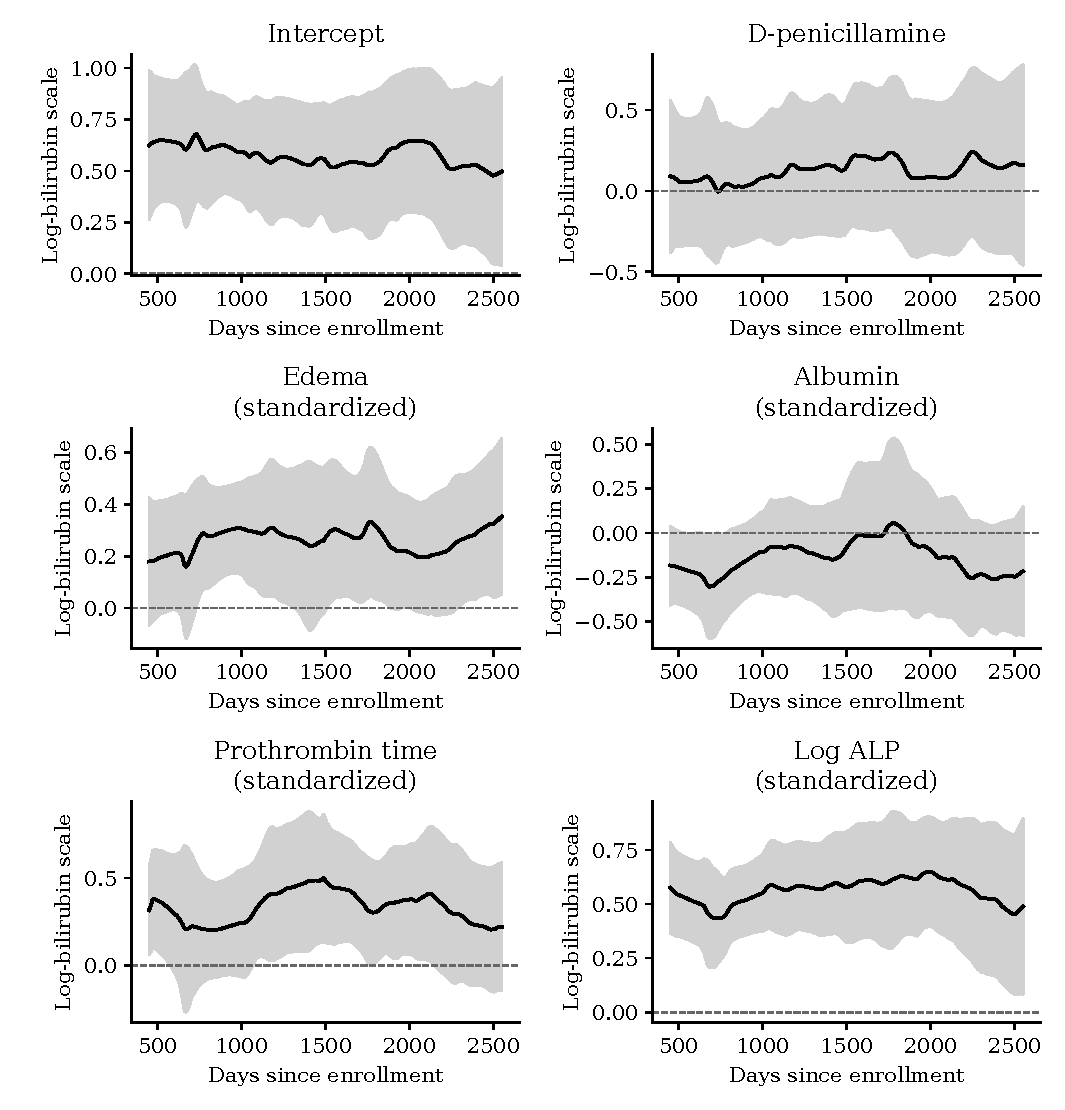
\includegraphics[width=\linewidth]{results/realdata/pbc_vcm_bands.pdf}
\caption{PBC coefficient estimates and nominal joint 95\% bands under the working model. Independent visit times and noninformative follow-up are not established for these data.}
\label{fig:pbc-vcm-new}
\end{figure}

In Figure~\ref{fig:pbc-vcm-new}, the treatment band contains zero throughout the displayed interval, while the log-ALP band remains above zero. Edema and prothrombin time have positive exclusions on portions of follow-up; albumin has short negative exclusions. Bandwidth factors 0.8 and 1.2 and a shorter 2,000-day horizon preserve the treatment and log-ALP descriptions but change the shorter exclusions. Full sensitivity results are in Section~\ref{app:numerics}. These are descriptive adjusted associations: conditioning on contemporaneous biomarkers does not identify a randomized treatment effect, and a band containing zero does not establish equivalence.
\FloatBarrier


\section{Discussion}\label{sec:discussion}

Subject contributions link local polynomial estimates to
Gaussian and bootstrap approximation without requiring
individual trajectory reconstruction. The bounds quantify the effects of
sampling frequency, dimension, smoothing bias, and estimation of the
design and residuals. Their explicit dimension dependence permits growing
VCMs. For high-dimensional means, a common fixed-size design allows
coordinatewise fitting without mixing response coordinates.
The resulting approximation and coverage bounds depend on dimension
through logarithmic factors and a maximum-coordinate tail envelope.
Uniform control of this envelope can yield logarithmic dimension
dependence even with polynomial tails; sub-Gaussian path suprema
provide another sufficient condition. Coordinate moments alone do
not imply such an improvement.

The explicit powers of $p$ in our bounds follow worst-case inequalities
under the stated assumptions. They account for mixing coordinate scores
through the inverse local design and accumulating coefficient errors in
fitted residuals. Designs with diagonal second-moment matrices or
fixed-size groups of correlated predictors can reduce these
dimension factors when the inverse-design absolute row sums remain
uniformly bounded. The stated dimension restrictions are therefore
sufficient conditions and need not be sharp.

The results assume error-free predictors and observation times independent
of the trajectories. They require a bandwidth satisfying the displayed
approximation and bias conditions. The numerical comparisons show that
moderate-sample joint undercoverage can remain. Extensions to informative
visits, measurement error in predictors, and justified finite-sample
corrections are therefore useful directions for further work.


\section*{Supplementary Material}
The supplementary document contains proofs, sampling-frequency and bandwidth results, the high-dimensional mean extension, and additional numerical and data-processing details. Reproduction code and complete simulation records accompany the manuscript.
\referencefont
\bibliographystyle{Chicago}
\bibliography{bibfile}

\bigskip
\noindent\begin{minipage}{\textwidth}
\noindent Haozhen Shu. National Institute of Education, Nanyang Technological University, Singapore.\\
E-mail: \href{mailto:haozhen.shu@nie.edu.sg}{haozhen.shu@nie.edu.sg}
\medskip

\noindent Zhenhua Lin. Department of Statistics and Data Science, National University of Singapore, Singapore.\\
E-mail: \href{mailto:linz@nus.edu.sg}{linz@nus.edu.sg}
\medskip

\noindent Yinan Lin. National Center for Applied Mathematics in Chongqing, Chongqing Normal University, Chongqing, China.\\
E-mail: \href{mailto:linyn@cqnu.edu.cn}{linyn@cqnu.edu.cn}
\end{minipage}
\end{document}
